\documentclass{scrreprt}

%Für deutsche Trennung
\usepackage[ngerman]{babel}
%Für UTF8-Codierung, mit Umlauten!
\usepackage[utf8]{inputenc}

%Für Links, auch innerhalb des Dokuments
\usepackage{hyperref}

%Einbinden von Grafiken
\usepackage{graphicx}

\usepackage{booktabs}

% Zusatzpakete verbatim und moreverb: listing-Umgebung
\usepackage{verbatim, moreverb}
\usepackage{color}
\definecolor{darkred}{rgb}{0.5,0,0}
\usepackage{listings}		%Für Quellcode

\tolerance=1000

\lstloadlanguages{Java, XML}
\lstset{language=Java}
\lstset{
basicstyle=\ttfamily, % alle listings scriptsize drucken (kann man gerade noch lesen) und Schreibmaschinenschrift für alles
keywordstyle=\color{darkred}\bfseries, % Schlüsselwörter fett und dunkelrot drucken
commentstyle=\color{blue}, % Kommentare blau drucken
showstringspaces=false, % Strings im Code ohne Kenntlichmachung von Leerzeichen
breaklines=true,
frame=lines,
numbers=left,
numberstyle=\tiny,
tabsize=3
}

\newcommand{\lstx}[1]{\lstinline$#1$} 


\title{Software Quality Measurement}
\author{Gruppe H}
\date{\today}

\begin{document}

\maketitle
\tableofcontents

\chapter{Software Quality Measurement}

Für \lstx{mallet}\footnote{\href{https://github.com/mimno/Mallet}{Mallet auf github}}, eine Verarbeitungssoftware für natürliche Sprache, sollen beispielhaft Kenngrößen für Softwarequalität ermittelt und ausgewertet werden. Zur Berechnung der Kenngrößen wird \lstx{ckjm}\footnote{\href{https://github.com/dspinellis/ckjm}{ckjm auf github},  \href{https://www.spinellis.gr/sw/ckjm/doc/indexw.html}{Manual}} verwendet, das alle sechs Kenngrößen (Metriken zum Messen von Softwarequalität) nach Chidamber and Kemerer sowie zwei zusätzliche ermittelt. Die Ausgaben von \lstx{ckjm} werden mit Hilfe eines zur Verfügung gestellten, auf \lstx{matplotlib} basierenden Pythonskripts aufbereitet und in Form von Histogrammen dargestellt.

\begin{lstlisting}[caption = Beispiele für den Output von mallet]
cc.mallet.extract.test.TestDocumentExtraction 7 0 0 20 31 21 0 7
cc.mallet.pipe.SerialPipes$Predicate 2 1 0 2 3 1 1 2
cc.mallet.classify.BalancedWinnowTrainer 6 0 0 11 21 11 1 6
cc.mallet.util.CharSequenceLexer 20 1 0 1 45 94 14 16
...
\end{lstlisting}


%TODO Output the 3 classes with the highest and lowest scores for the measures CBO and LCOM. (You may use the provided file findExtremes.py for doing this) Have a look at those classes, why do they have high/low scores for CBO and LCOM? How do you judge the quality of the classes and the effectiveness of the measures? Write a short explanation. 

\section{CBO - Kopplung zwischen Objektklassen}


\begin{figure}
 \centering
 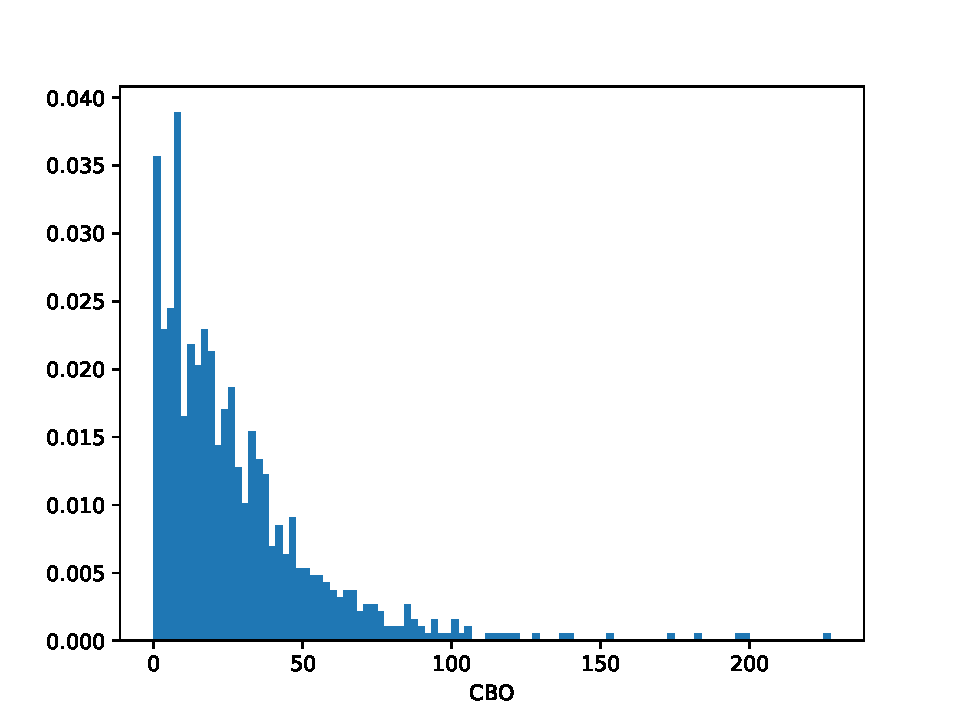
\includegraphics[width=.8\textwidth]{./CBO.pdf}
 % CBO.pdf: 0x0 pixel, 300dpi, 0.00x0.00 cm, bb=
 \caption{CBO: Coupling between Object Classes}
 \label{abb:cbo}
\end{figure}

Ein hoher Wert des CBO (Coupling between object classes) ist erwünscht. Das bedeutet, dass Methoden mit vielen Instanzvariablen eng gekoppelt sind, was sich wiederum positiv auf die Softwarequalität auswirkt.

% The coupling between object classes (CBO) metric represents the number of classes coupled to a given class (efferent couplings, Ce). This coupling can occur through method calls, field accesses, inheritance, arguments, return types, and exceptions.



Ein kleiner Wert ist unerwünscht, da dies bedeutet, dass alle Methoden der Klasse eigene unabhängige Instanzvariablen benutzen. Dies wirkt sich negativ auf die Softwarequalität aus. Über 10\% der Klassen haben einen CBO von 0, die Tabelle der schlechtesten Klassen zeigt also nur eine Teilmenge der Klassen mit diesem Wert.



\begin{center}
\begin{tabular}{ll}
\toprule
CBO: schlechteste Klassen\\
\midrule
\lstx{cc.mallet.util.Lexer} & 0\\
\lstx{cc.mallet.topics.TopicReports} & 0\\
\lstx{cc.mallet.cluster.util.PairwiseMatrix} & 0 \\
\bottomrule
\end{tabular}
\end{center}


\begin{center}
\begin{tabular}{ll}
\toprule
CBO: beste Klassen\\
\midrule
\lstx{cc.mallet.classify.tests.TestNaiveBayes} & 33 \\ 
\lstx{cc.mallet.fst.semi_supervised.tui.SimpleTaggerWithConstraints} & 34 \\
 \lstx{cc.mallet.fst.tests.TestCRF}& 51 \\
\bottomrule
\end{tabular}
\end{center}



Das Histogramm (Abb. \ref{abb:cbo}) zeigt die CBO-Werte aller getesteten Klassen. Die CBO-Werte liegen im Bereich von 0 bis 51.

\section{LCOM - Mangel an Abgeschlossenheit}

Im Vergleich zum CBO-Wert verhält sich der LCOM-Wert komplementär. Ein hoher Wert steht für den Mangel an Kohäsion (Zusammenhang zwischen den Methoden) und wirkt sich somit negativ auf die Softwarequalität aus.
Ein niedriger Wert bedeutet keinen Mangel und ist somit positiv für die Softwarequalität.

\begin{figure}
 \centering
 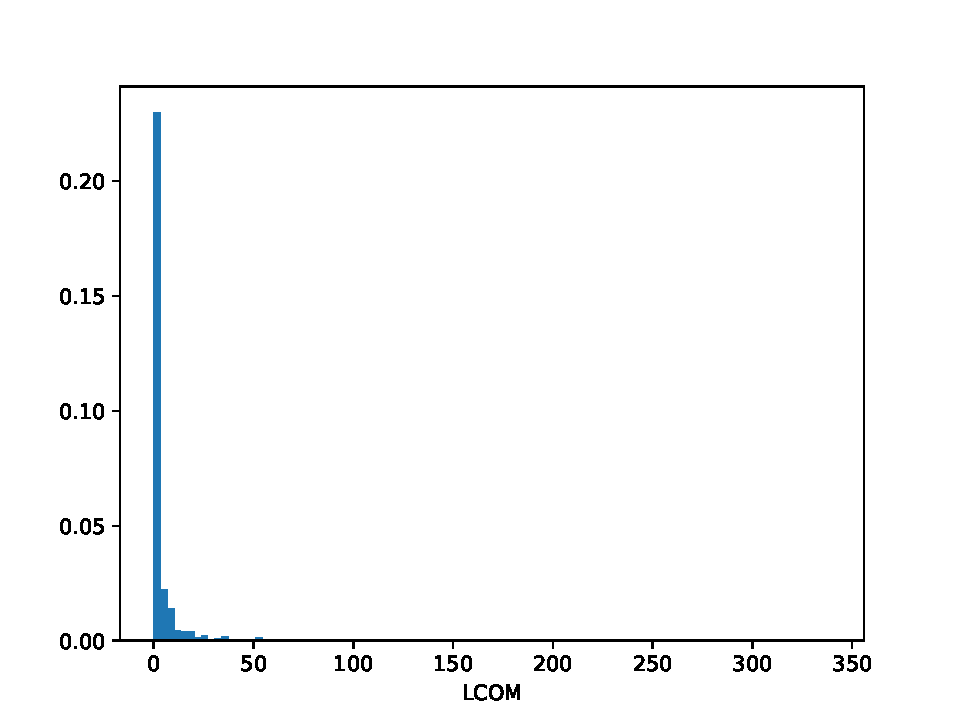
\includegraphics[width=.8\textwidth]{./LCOM.pdf}
 % LCOM.pdf: 0x0 pixel, 300dpi, 0.00x0.00 cm, bb=
 \caption{LCOM: Lack of cohesion in methods}
 \label{abb:lcom}
\end{figure}


\begin{center}
\begin{tabular}{ll}
\toprule
LCOM: beste Klassen\\
\midrule
\lstx{cc.mallet.fst.semi_supervised.GELatticeTask} &0 \\
\lstx{cc.mallet.optimize.OptimizerEvaluator\$ByBatchGradient} &0 \\
\lstx{cc.mallet.util.ProgressMessageLogFormatter} &0  \\
\bottomrule
\end{tabular}
\end{center}


\begin{center}
\begin{tabular}{ll}
\toprule
LCOM: schlechteste Klassen \\
\midrule
\lstx{cc.mallet.types.InstanceList} & 2365\\
\lstx{cc.mallet.types.MatrixOps} & 1911\\
\lstx{cc.mallet.fst.CRF} & 1578 \\
\bottomrule
\end{tabular}
\end{center}


\section{Weitere Kenngrößen und graphische Darstellung}

%TODO 7. Plot a histogram for each of the measures using matplotlib. (You may use the provided file findExtremes.py for doing this) What insights do you gain from these plots concerning the Mallet repository? You may compare the repository to other repositories of your choosing.

Die Kenngrößen werden als normierte Histogramme dargestellt, auf der x-Achse sind Bereiche möglicher Werte der Kenngröße aufgetragen. Auf der y-Achse der Anteil der Klassen, die diesem Wertebereich zugeordnet sind.

Neben den in den vorherigen Kaptieln bereits vorgestellten Kenngrößen wurden folgende weitere von \lstx{ckjm} ermittelt:

\begin{description}

% A class's weighted methods per class WMC metric is simply the sum of the complexities of its methods. As a measure of complexity we can use the cyclomatic complexity, or we can abritrarily assign a complexity value of 1 to each method. The ckjm program assigns a complexity value of 1 to each method, and therefore the value of the WMC is equal to the number of methods in the class.

%TODO Ich habe ein paar Klassen aufgemacht und alle Methoden gezählt, das passt nicht immer. Steht irgendwo was von einem Kriterium, welche Meothden zählen und welche nicht?
\item [WMC: Weighted methods per class] (Abb. \ref{abb:wmc} li.) stellt der Wert einfach nur die Anzahl der Methoden einer Klasse dar, weil die Gewichtung (entsprechend der Komplexität) aller Methoden auf 1 gesetzt wurde. Als Grund für diesen festen Wert werden die einfache Implementierung und die Kompatibilität zu Chidamber und Kemerer genannt. Für die Verständlichkeit und Erweiterbarkeit ist es von Vorteil, wenn die Anzahl der Methoden einer Klasse in einem überschaubaren Rahmen bleiben. Bei der betrachteten Software haben alle Klassen 0–5 Methoden, was sehr überschaubar ist.  

Größere Werte sind negativ. Kleinere Werte sind positiv.

    
    
% Depth of Inheritance Tree
% The depth of inheritance tree (DIT) metric provides for each class a measure of the inheritance levels from the object hierarchy top. In Java where all classes inherit Object the minimum value of DIT is 1.

%TODO Wir haben Bäume der Tiefe 0, das sollte aber laut Manual nicht möglich sein.

\item [DIT: Depth of Inheritance Tree] (Abb. \ref{abb:wmc} re.)
 DIT misst die Tiefe des Vererbungsbaums. Je tiefer dieser Baum ist, desto negativer wirkt sich das auf die Softwarequalität aus, weil es dann schwieriger ist, die Vererbungsstruktur bis in die Blätter nachzuvollziehen. D.h. in unserem Histogramm sind solche Klassen gut, die den Wert 0 haben, weil die Tiefe des Baums


    
    
    
\item [NOC: Number of Children] (Abb. \ref{abb:noc_rfc} li.)
    NOC misst die Anzahl der Subklassen, die direkt unter der gemessenen Klasse existieren. Ein hoher Wert bedeutet, dass diese Klasse oft wiederverwendet wird und somit Code gespart wird. Das bedeutet aber auch, dass eine Klasse mit hohem Wert gut getestet muss, um die Softwarequalität zu steigern. Im Vergleich zu DIT misst NOC die Breite des Baums, statt der Tiefe.


    
    
\item [RFC: Response for a Class] (Abb. \ref{abb:noc_rfc} re.)
    steht für die Anzahl aller möglichen auszuführenden Methoden innerhalb der Klasse. Je höher der Wert, desto höher die Komplexität der Klasse. Also ist ein hoher Wert nicht erwünscht.

    
% A class's afferent couplings is a measure of how many other classes use the specific class. Ca is calculated using the same definition as that used for calculating CBO (Ce).    
    
\item [Ca: Afferent coupling] (nicht C\&K-Metrik, Abb. \ref{abb:ca_npm} li.)
    gibt an, wie viele Klassen von dieser Klasse abhängen. Eine Klasse mit einem hohen Ca-Wert hat eine hohe Verantwortung innerhalb der Software, weil sie Funktionalitäten für viele andere Klassen zur Verfügung stellt. 
    Weit über die Hälfte der Klassen in \lstx{mallet} weist hier eher geringe Werte unter 10 auf. Es gibt aber auch mehrere Klassen, die von über 20 und bis zu 68 anderen Klassen genutzt werden, das heißt dass eine Änderung einer dieser Klassen in sehr vielen anderen Klassen Auswirkungen haben kann. Diese Auswirkungen sind extrem schlecht zu überschauen, die Bearbeitung einer solchen Klasse führt zu nicht abschätzbaren Folgen und jeden abhängige Klasse bringt ein weiteres Risiko, dass die Software nicht mehr funktioniert, mit sich.
    %\begin{itemize}
    %\item Der Ca Wert bestimmt die Anzahl der Packages, die von der Package dieser Klasse abhängen. Ein hoher Wert bedeutet eine hohe Verantwortung für diese Package und ist somit negativ behaftet. Da unsere Klassen größtenteils niedrigere Werte besitzen, ist dies positiv für die Softwarequalität.
    %\end{itemize}

%TODO @Rebecca: Bitte nochmal bewerten, ob das so richtig ist. Ich würde ja eher die Definition von der Seite nehmen, siehe unten.
% The NPM metric simply counts all the methods in a class that are declared as public. It can be used to measure the size of an API provided by a package.
\item [NPM: Number of Public Methods for a class] (nicht C\&K-Metrik, Abb. \ref{abb:ca_npm} re.)
 bestimmt die Anzahl der public methods innerhalb der Klasse. Sie ist ein Maß dafür, wie umfangreich die API ist, die eine Klasse, bzw. in Summe ihr Package zur Verfügung stellt. Öffentliche Methoden sollten bewusst und sparsam eingesetzt werden, sie brauchen eine gute Dokumentation und dürfen in ihre nach außen sichtbare Funktionalität darf nicht ohne Weiteres verändert werden. Sie stellen also ein Hindernis für Veränderungen in der Klasse dar und erschweren ihre Wartung.
 Ein  hoher Wert für NPM kann ein Hinweis darauf sein, dass das Prinzip der Kapselung von Klassen nicht eingehalten wurde. 
 %Ein hoher Wert bedeutet eine große Verantwortung und hohe Komplexität und ist daher für die Softwarequalität nicht von Vorteil.



\end{description}

\begin{figure}
 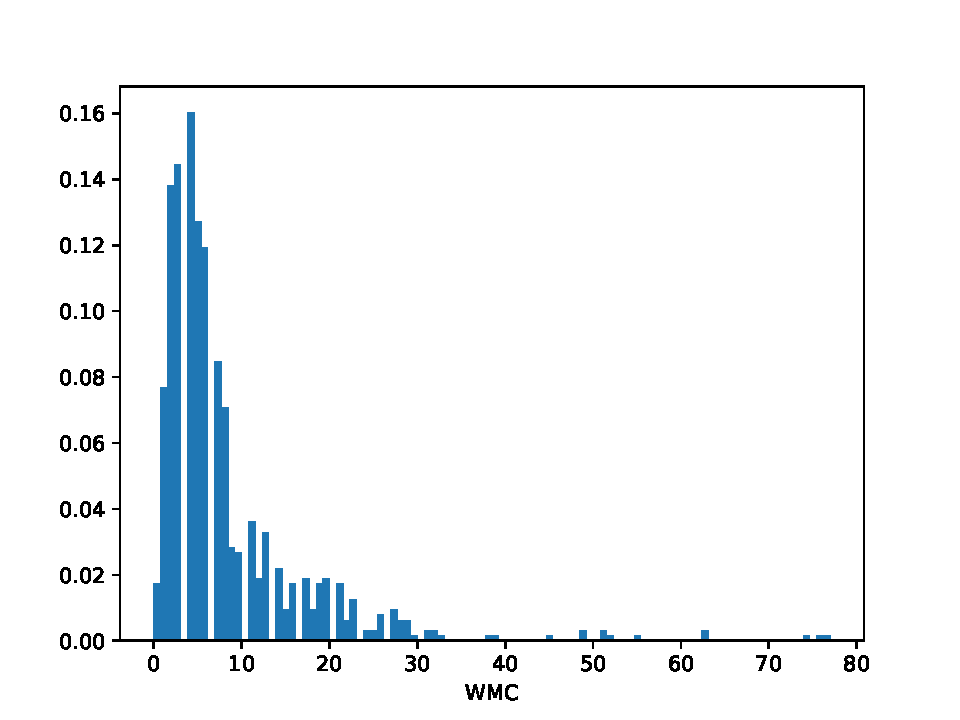
\includegraphics[width=.45\textwidth]{./WMC.pdf}
 % WMC.pdf: 0x0 pixel, 300dpi, 0.00x0.00 cm, bb=
  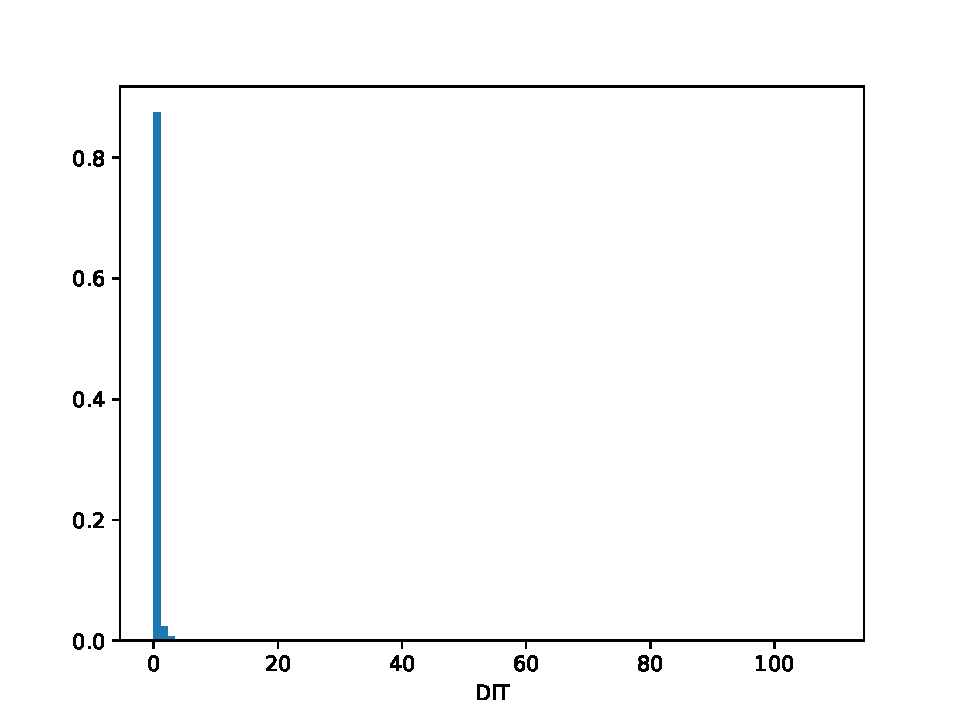
\includegraphics[width=.45\textwidth]{./DIT.pdf}
 \caption{WMC (WB: 0-5) und DIT (WB: 0-109)}
 \label{abb:wmc}
\end{figure}

% Depth of inheritance tree (DIT)
% This represents the number of discrete levels in the inheritance tree where
% subclasses inherit attributes and operations (methods) from superclasses. The
% deeper the inheritance tree, the more complex the design. Many object classes
% may have to be understood to understand the object classes at the leaves of the
% tree.

\begin{figure}
 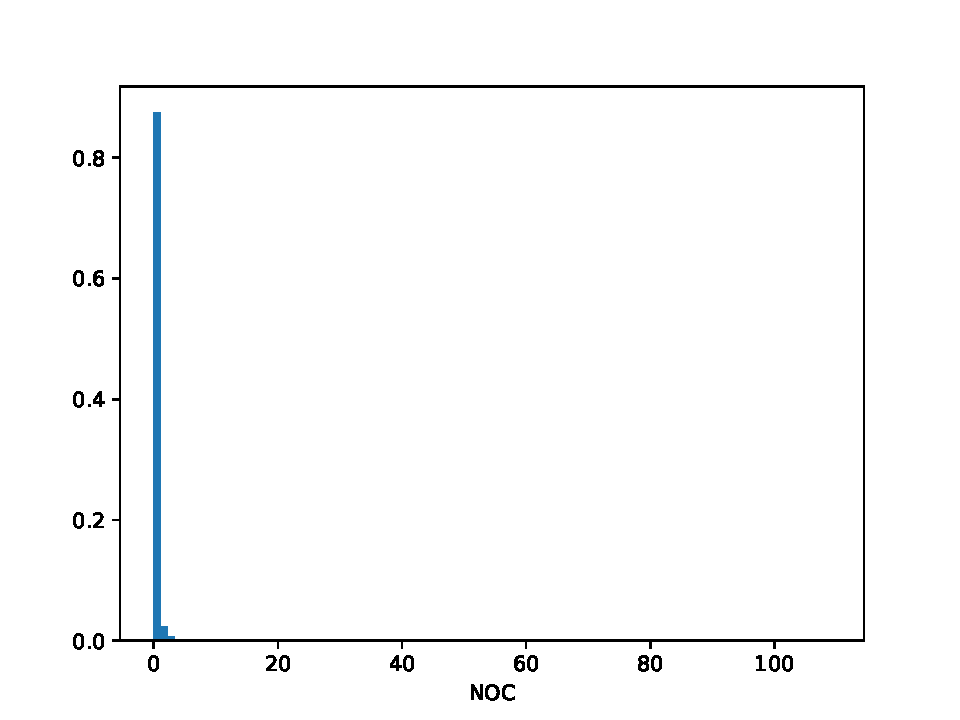
\includegraphics[width=.45\textwidth]{./NOC.pdf}
 % WMC.pdf: 0x0 pixel, 300dpi, 0.00x0.00 cm, bb=
  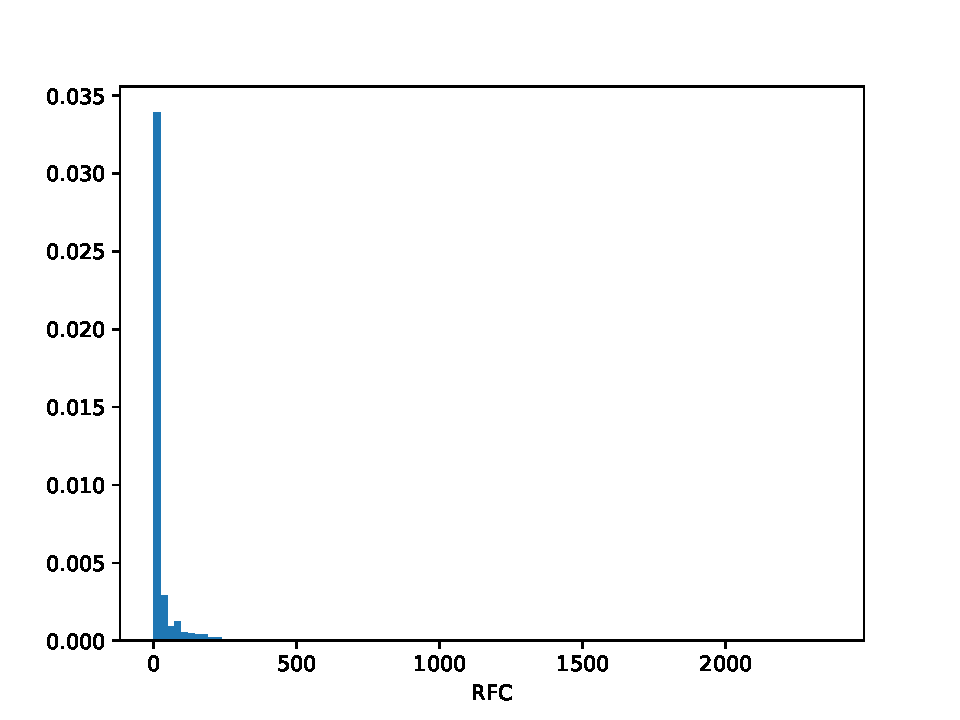
\includegraphics[width=.45\textwidth]{./RFC.pdf}
 \caption{NOC (WB: 0–51) und RFC (WB: 0–2356)}
 \label{abb:noc_rfc}
\end{figure}

% Number of children (NOC)
% This is a measure of the number of immediate subclasses in a class. It measures
% the breadth of a class hierarchy, whereas DIT measures its depth. A high value
% for NOC may indicate greater reuse. It may mean that more effort should be
% made in validating base classes because of the number of subclasses that
% depend on them.

\begin{figure}
 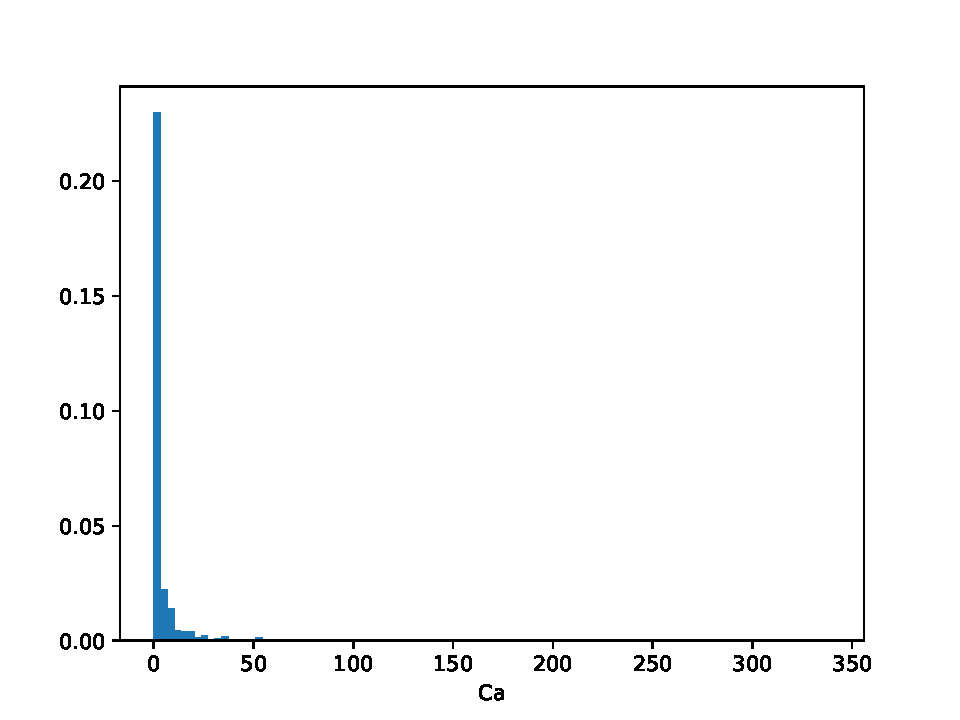
\includegraphics[width=.45\textwidth]{./Ca.pdf}
 % WMC.pdf: 0x0 pixel, 300dpi, 0.00x0.00 cm, bb=
  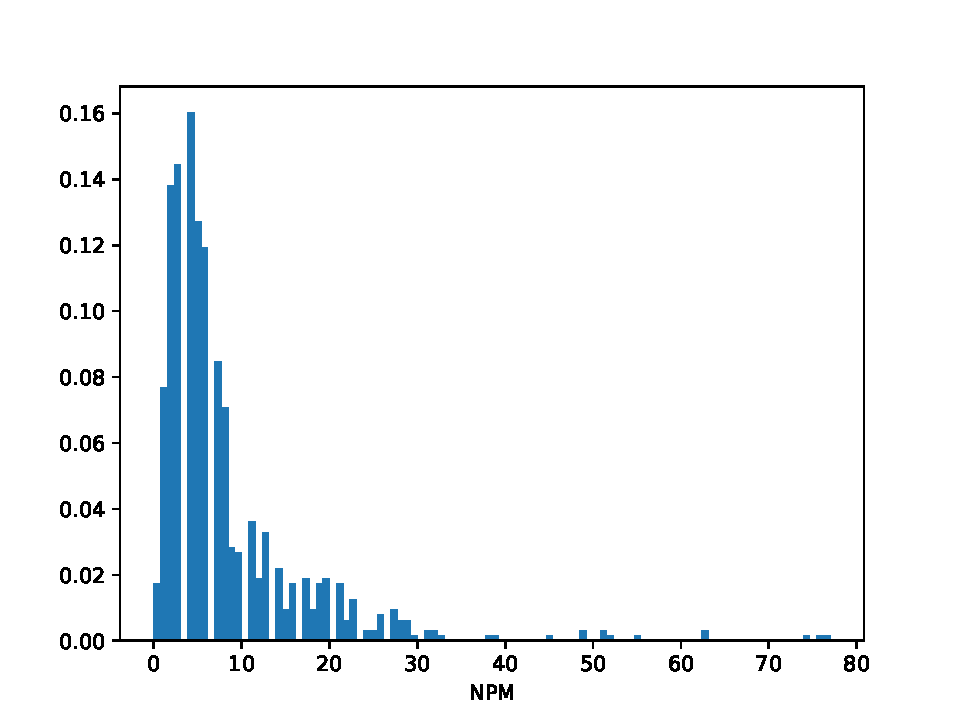
\includegraphics[width=.45\textwidth]{./NPM.pdf}
 \caption{Ca (WB: 0-68) und NPM (0-77)}
 \label{abb:ca_npm}
\end{figure}


\section{Vergleich mit einer abgeänderten Version von mallet}

Dem Programm \lstx{mallet} werden zwei weitere Klassen \lstx{NewParallelTopicModel.java} und \lstx{TopicInferencerInterface.java} hinzugefügt. Nach dem Kompilieren wird die Analyse von \lstx{mallet} wiederholt und es werden die Kennzahlen der Klassen \lstx{NewParallelTopicModel} und \lstx{ParallelTopicModel} verglichen:

%TODO 8. In the package cc.mallet.topics there is a class called ParallelTopicModel which is used to learn a model on some data. A different class in the same package, called TopicInferencer, is used for the evaluation of the trained model. Add the provided Java files to this package and rebuild Mallet. Now compare the output of CKJM on ParallelTopicModel and NewParallelTopicModel. What do the new values indicate? What is the difference between the two classes?


\begin{center}
\begin{tabular}{lllllllll}
\toprule
Klasse & WMC & DIT & NOC & CBO & RFC & LCOM & Ca & NPM \\
\midrule
\lstx{NewParallelTopicModel} & 68 & 1 & 0 & 22 & 233 & 800 & 0 & 61 \\
\lstx{ParallelTopicModel} & 63 & 1 & 2 & 21 & 227 & 627 & 11 & 58 \\
\bottomrule
\end{tabular}
%TODO Diese Tabelle muss noch beschrieben werden, ich hab keine Ahnung davon :/ – Das ist ungünstig.
\end{center}

Im Vergleich zur ursprünglichen Version der von \lstx{ParallelTopicModel} hat sich WMC um den Wert 5 erhöht, das heißt die Anzahl der Methoden der Klasse hat zugenommen, der um 3 erhöhte Wert für NPM zeigt, dass davon nur 3 Methoden public waren. Die Tiefe des Vererbungsbaums (DIT) ist unverändert, die Anzahl der Kinder (NOC) um 2 auf 0 verringert. Die Kopplung zwischen Objektklassen (CBO) hat sich kaum verändert, während der Mangel an Abgeschlossenheit (LCOM) um über 25\% angewachsen ist. Der Ca-Wert, der die Anzahl der Klassen, die von dieser Klassen abhängen, angibt, hat sich laut Berechnung von 11 auf 0 reduziert. %Wie auch immer das funktionieren soll...


\end{document}
